\chapter{Architektura}
\label{cha:architektura}

Ogólna architektura zaimplementowanego rozwiązania została zaprezentowana na rysunku \ref{fig:ogolna-architektura}.
\begin{figure}[!htb]
    \centerline{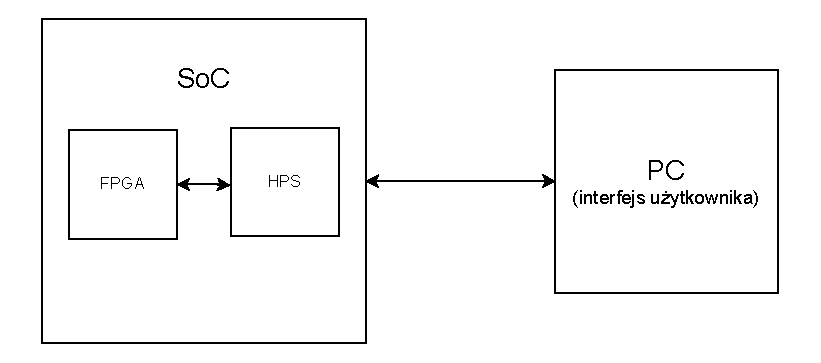
\includegraphics[scale=0.9]{system.pdf}}
    \caption{Diagram przedstawiający uproszczoną architekturę systemu}
    \label{fig:ogolna-architektura}
\end{figure}

\section{Platforma}
\label{sec:platforma}
Platformą wybraną do realizacji pracy jest system heterogeniczny DE0-Nano-SoC, którego glównym elementem był układ Intel Cyclone V SoC.Zawiera on \ac{fpga} oraz \ac{hps} oparty na procesorze \acs{arm}, co umożliwia podział zadań między hardware i software.

Układ \ac{fpga} w Cyclone V SoC oferuje programowalne zasoby, takie jak \ac{lut}, bloki \ac{dsp} oraz pamięci RAM, które umożliwiają implementację szerokiego zakresu funkcji, od prostych operacji po bardziej zaawansowane algorytmy. Zintegrowany z \ac{fpga} system \ac{hps}, oparty na dwurdzeniowym procesorze ARM Cortex-A9 z zegarem 925 MHz, komunikuje się z \ac{fpga} za pomocą mostków AXI i AXI Lightweight.

Decyzja o wyborze tej konkretnej platformy była podyktowana kilkoma istotnymi aspektami. Przede wszystkim heterogeniczna architektura systemu, dobrze sprawdza się w zastosowaniach \ac{dsp}, co opisano dokładniej w sekcji \ref{sec:system-heterogeniczny}.

Ponadto układ posiada gniazdo na kartę micro SD, na którą można wgrać obraz całego systemu. Karta SD pełni funkcję głównego nośnika, z którego ładowany jest system przy starcie. Dzięki wykorzystaniu wbudowanego slotu możemy uruchomić procesor wykorzytując niemal każdy system operacyjny wspierający architekturę ARM, a korzystając z narzędzi takich jak \hyperref[sec:linux-embedded]{Yocto} jesteśmy w stanie skonfigurować system zgodnie z naszymi wymaganiami.

% Innym istotnym elementem, który umożliwił połączenie sieciowe, a co za tym idzie implementację zdalnego interfejsu użytkownika było wbudowane złącze Ethernet.
Złącze Ethernet w układzie zapewnia dostep do połaczenia sieciowego, co umożliwia zdalne zarządzanie oraz wymianę danych między systemem a zewnętrznymi urządzeniami. W kontekście opisywanej architektury, interfejs został wykorzystany, aby umożliwić połączenie sieciowe niezbędne do komunikacji z zaprojektowaną aplikacją internetową.

\begin{figure}[!htb]
    \centerline{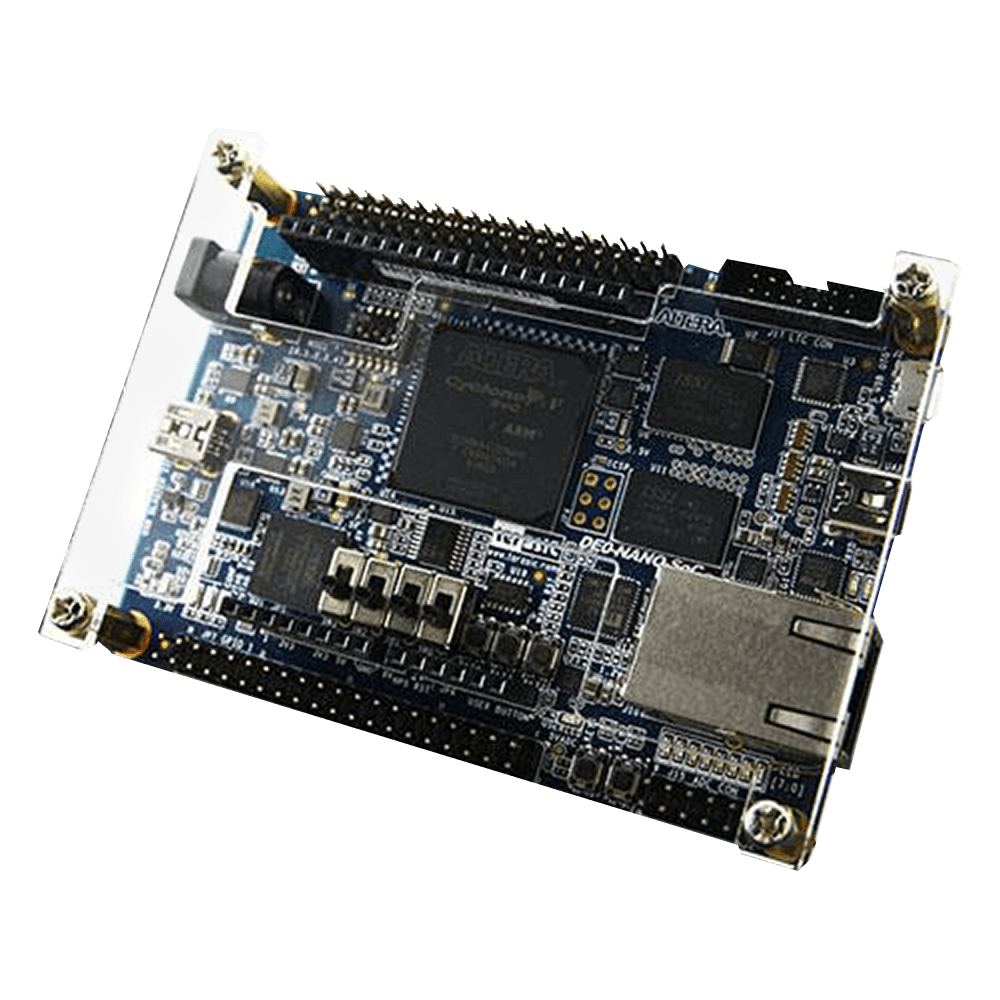
\includegraphics[scale=0.2]{de0-nano-soc.png}}
    \caption{Układ DE0-Nano-SoC (Cyclone V)}
    \label{fig:de0-nano-soc}
\end{figure}

Ze względu na przystępną cenę i elastyczność konfiguracji,
układ ten znajduje szerokie zastosowanie w projektach wymagających kompromisu między wydajnością a kosztami, szczególnie w środowiskach akademickich. Niniejsza praca zawiera przykłady tego, jak efektywnie wykorzystać ten układ w implementacji algorytmów przetwarzania sygnałów.

\section{Architektura Sprzętowa}
\label{sec:architektura-hw}

Architektura sprzętowa systemu została zaimplementowana z wykorzystaniem układu \ac{fpga}, który pełni rolę centralnego komponentu przetwarzającego dane. Rysunek \ref{fig:uproszczony-schemat-hw} przedstawia uproszczoną architekturę systemu, ukazującą główne jego elementy. System składa się z dwóch pamięci \ac{ocm}, z których jedna jest odpowiedzialna za przechowywanie danych wejściowych przekazywanych z \ac{hps}, natomiast druga - danych wyjściowych po przetworzeniu.

Dane wejściowe są przesyłane do modułu \ac{dsp} za pomocą kontrolera DMA i interfejsu ST-MM. Cała transmisja przez moduł \ac{dsp} odbywa się w sposób strumieniowy, co oznacza, że zarówno dane wejściowe, jak i wyjściowe są przesyłane w czasie rzeczywistym. W module \ac{dsp} realizowane są operacje przetwarzania sygnałów, w tym filtracja przy użyciu filtru \ac{fir} oraz szyfrowanie danych. Przetworzone dane są przesyłane do drugiej pamięci \ac{ocm} poprzez interfejs MM-ST, skąd mogą zostać odczytane przez hosta.

\begin{figure}[!htb]
    \centerline{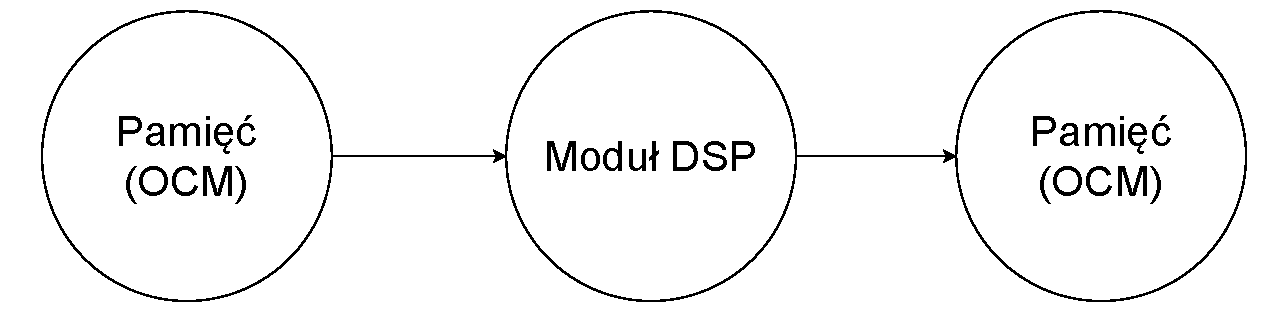
\includegraphics[scale=0.5]{uproszczonySchematHW.pdf}}
    \caption{Diagram przedstawiający architekturę sprzętową}
    \label{fig:uproszczony-schemat-hw}
\end{figure}

\subsection{Interfejsy}
W systemie wykorzystano dwa interfejsy do transmisji danych: \ac{avmm} oraz \ac{avst}.

Avalon MM jest interfejsem pamięciowym, który sprawdza się w sytuacjach, gdy zachodzi potrzeba bezpośredniego odczytu lub zapisu danych do pamięci. Umożliwia transfer w postaci tzw. burstów, co oznacza, że pozwala na przesyłanie wielu paczek danych w kolejnych taktach zegara.

Avalon Streaming pozwala na przesył danch w sposób ciągły bez konieczności adresacji każdej paczki. Interfejs sprawdza się aplikacjach bazuących na przetwarzaniu w czasie rzeczywistym, wymagających szybkiego transferu dużych ilości danych.

Wybór pomiędzy tymi interfejsami zależy od specyficznych potrzeb aplikacji -- Avalon MM jest odpowiedni do operacji bazujących na transakcjach do pamięci, podczas gdy Avalon Streaming lepiej sprawdza się w przypadku transmisji danych pomiędzy modułami, które mają je przetworzyć.

\subsection{Zaprojektowane moduły \ac{dsp}}
System został wyposażony w dwa moduły \ac{dsp} -- filtr FIR o zmiennych współczynnikach oraz moduł szyfrowania danych oparty na algorytmie \ac{tea}.

Moduł filtru FIR umożliwia dynamiczną zmianę współczynników z poziomu oprogramowania, co pozwala na realizację różnych typów filtracji sygnałów w czasie rzeczywistym. Dzięki tej funckjonalności, filtr może pełnić różne typy filtracji, takie jak:

\begin{itemize}
    \item Low Pass (dolnoprzepustowy): Wygładzanie sygnału przez eliminację wysokich częstotliwości.
    \item Bandpass (pasmowoprzepustowy): Przepuszczanie sygnałów z określonego zakresu częstotliwości.
    \item Moving Average (średnia krocząca): Wygładzanie danych poprzez uśrednianie kolejnych wartości sygnału.
\end{itemize}

Modularność współczynników filtru umożliwia dostosowanie parametrów filtracji w zależności od aktualnych wymagań aplikacji, co znacząco zwiększa przydatność modułu w różnych zastosowaniach.

Moduł enkrypcji oparty na algorytmie \ac{tea} zapewnia bezpieczne szyfrowanie danych w systemie. \ac{tea} jest lekkim algorytmem szyfrowania blokowego, którego najważniejszymi cechami są prostota implementacji oraz wysoka prędkość przetwarzania. Algoytm operuje na danych wejściowych o szerokości 32 bitów (w zaimplementowanym systemie szerokość wejść została ograniczona do 32 bitów) i 128-bitowym kluczu. Ze względu na swoją prostotę i niskie zapotrzebowanie na zasoby, TEA jest idealnym wyborem do zastosowań, w których wymagana jest efektywność przy zachowaniu podstawowego poziomu bezpieczeństwa.




% Układ \ac{fpga} w Cyclone V SoC zawiera programowalne zasoby, takie jak \ac{lut}, bloki \ac{dsp}
% oraz wewnętrzne pamięci RAM. Te zasoby pozwalają na realizację szerokiego zakresu funkcji, od prostych operacji po złożone algorytmy przetwarzania sygnałów.
% \ac{fpga} może być dynamicznie rekonfigurowany, co zapewnia elastyczność w projektowaniu systemów sprzętowych.

% HPS w Cyclone V SoC to zintegrowany system oparty na dwurdzeniowym procesorze ARM Cortex-A9 oferującym zegar 925MHz. Procesor może funkcjonować niezależnie,
% jednak w praktyce jest on wykorzystywany do zarządzania zadaniami w \ac{fpga}, z którą komunikacja odbywa się pomocą mostków AXI/AXI Lightweight.







\newpage
\section{Architektura Programowa}
\label{sec:architektura-sw}




% \begin{figure}[!htb]
%     \centerline{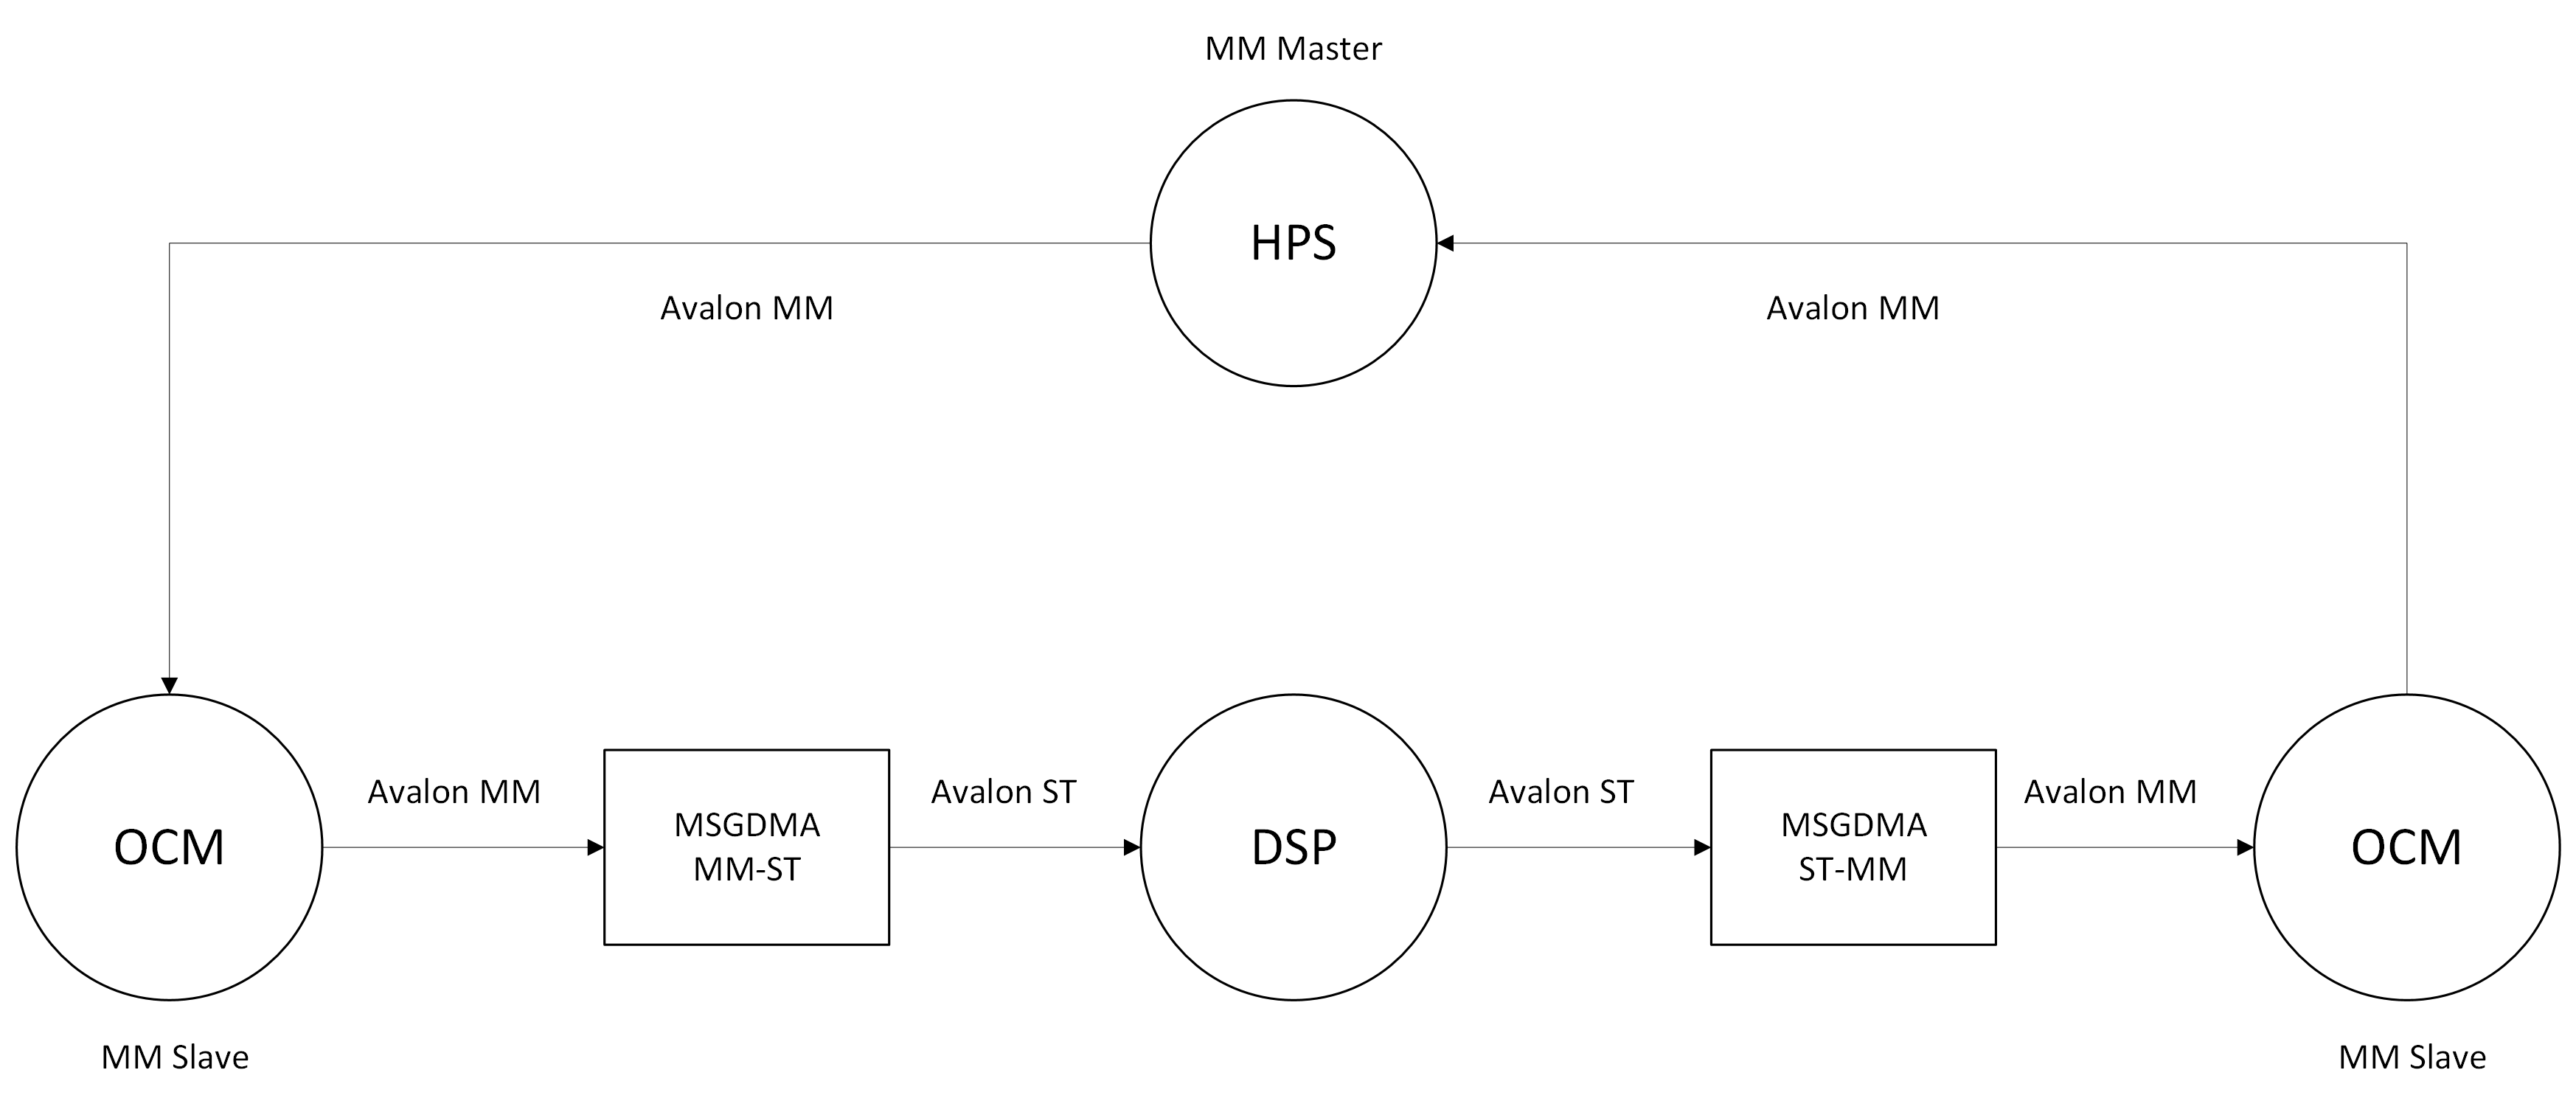
\includegraphics[scale=0.5]{hardwareSystemDiagram.png}}
%     \caption{Diagram przedstawiający architekturę sprzętową systemu}
%     \label{fig:architektura-hw}
% \end{figure}